\documentclass[a4paper, USenglish, cleveref, autoref, thm-restate]{lipics-v2021}

\bibliographystyle{plainurl}

\usepackage[T1]{fontenc} 
\usepackage[utf8]{inputenc}
\usepackage{graphicx}
\usepackage{amsmath}
\usepackage{amssymb}
\usepackage{amsthm}
\usepackage[ruled,linesnumbered,vlined]{algorithm2e}
\usepackage{xcolor}
\usepackage{tabularx}
\usepackage{tabu}
\usepackage{todonotes}
\usepackage{tabto}
%\usepackage{url}
\usepackage{hyperref}
\usepackage{caption} 

\usepackage{mathtools}
\DeclarePairedDelimiter\ceil{\lceil}{\rceil}
\DeclarePairedDelimiter\floor{\lfloor}{\rfloor}
\DeclareMathOperator\hi{\ensuremath{\mathsf{hi}}}
\DeclareMathOperator\lo{\ensuremath{\mathsf{lo}}}

\theoremstyle{definition}
\newtheorem{encoding}{Encoding}[section]


\title{Explaining SAT Benchmark Classifiers with Prime~Implicants}
\author{Markus Iser}{Karlsruhe Institute of Technology (KIT), Institute of Theoretical Informatics, Algorithm Engineering, Germany \and \url{https://algo2.iti.kit.edu/english/3986.php}}{markus.iser@kit.edu}{https://orcid.org/0000-0003-2904-232X}{}
\Copyright{Markus Iser}
\authorrunning{M. Iser}
\ccsdesc{Theory of computation~Logic and verification}
\ccsdesc{Computing methodologies~Supervised learning by classification}
\keywords{Benchmarks, Explainable Algorithm Selection, Prime Implicants}

\begin{document}
\maketitle
\begin{abstract}
Taxonomies for benchmark instances can be derived in several ways. For example, this can be based on their theoretical properties, or it can be based on their origin, e.g., a concrete application. 
Some algorithm selectors even generate instance classes based on a set of features in an unsupervised manner. 
We see a gap in the explainability of such approaches. 
In this paper, we present a SAT encoding for decision tree and random forest classifiers that we can use to generate prime implicants. 
We then apply this encoding to generate minimal explanations for two types of classifiers. 
The first type of classifier was trained to map SAT instances to their instance family.
The second type of classifier was trained as an instance-specific SAT solver selector on a small portfolio.
We show that the explainability of machine learning methods is useful for interpreting experiments as it provides valuable feedback to the algorithm developer.
\end{abstract}


%%%%%%%
\section{Introduction}

Models created by inductive learning algorithms are useful in practice.
The explainability of such automatically generated models is the subject of current research projects~\cite{Audemard:2021:Intelligibility, Darwiche:2020:Reasons}.
In particular, in applications for which accountability concerns arise, it is imperative that what is learned can be explained~\cite{Percy:2021:Accountability}. 

Automatic generation of explanations for machine-learned models requires to formalize those models. 
The symbolic representation of what is learned facilitates the application of deductive methods for reasoning about what is learned.
Deductive reasoning about inductively generated models is usually referred to by the term eXplainable AI (XAI)~\cite{Arrieta:2019:XAI}. 

The term \emph{explanation} is ambiguous. 
There is a plethora of possible formalizations leading to different definitions of explainability. 
Audemard et al. analyze the complexity of different kinds of XAI queries, among which are also prime implicants~\cite{Audemard:2020:XAI}. 
One of the explanation queries they analyze is prime implicants, which are also known as sufficient reasons~\cite{Darwiche:2020:Reasons}. 
Choi et al. present an encoding of decision tree and random forest classifiers for computing prime implicants~\cite{Choi:2020:RF}. 
However, they report on limitations of their approach when encoding cardinality constraints for multivalued variables. 

Inductive learning methods have been used in various ways to solve SAT instances more efficiently. 
Cherif et al. successfully use reinforcement learning to control the switching of branching heuristics~\cite{Cherif:2021:KissatMAB}. 
Soos et al. present clause forgetting heuristics based on supervised learning~\cite{Soos:2019:CrystalBall}. 
Prediction models have also been used to create algorithm selectors for portfolios of SAT solvers (cf. SATzilla~\cite{Xu:2008:SATzilla}). 
In their approach known as instance-specific algorithm configuration (ISAC), Kadioglu et al. use unsuperived learning to create clusters in the feature space of SAT instances~\cite{Kadioglu:2010:ISAC}. 
For each cluster, a configurator optimizes a SAT solver for the instances in that cluster. 

Prediction models for algorithm selection in SAT induce, in a sense, a taxonomy for SAT instances. 
This differs from the classes used in common practice, where instances are usually assigned to an instance family~\cite{Froleyks:2021:SC2020}. 
The instance family may for example describe a category of SAT applications (such as \textsf{hardware verification}), or refer to a specific class of instances that is of theoretical interest (such as \textsf{pigeon hole}). 

Elffers et al. analyze SAT solver configurations for instance classes of theoretical interest~\cite{Elffers:2018:Insights}. 
Audemard and Simon devise instance classes based on solver runtime parameters, and then they suggest class specific solver configurations~\cite{Audemard:2016:Extreme}. 

Given the circumstances sketched so far, we conclude that explanations of prediction models for SAT benchmarks can provide valuable feedback to the algorithm engineer about what was learned. 
Such explanations allow the algorithm engineer to reason about the induced instance taxonomy, and to improve their algorithm or configuration choices. 

In this paper, we present a propositional, conjunctive normal form (CNF) encoding of decision tree classifiers and random forests. 
The formula which we encode resembles a \emph{monotonic} combinatorial circuit, which makes it easy to compute prime implicants for it by using an off-the-shelf incremental SAT solver. 
We present a tool which can encode decision tree and random forest classifiers generated with the Python package \verb!scikit-learn!~\cite{Pedregosa:2011:Scikit} into propositional formulas. 
Our tool uses the SAT solver \verb!CaDiCaL!~\cite{Biere:2020:Cadical} via its \verb!IPASIR!~\cite{Balyo:2016:Ipasir} interface to generate prime implicants. 
All prime implicants are decoded into the minimal set of case-distinctions in the features space which they represent. 
We evaluate our tool on classifiers for SAT instances and show that prime implicants deliver concise explanations of classifier decisions. 

The document is structured as follows. 
In Section~\ref{sec:prelim}, we present a formalization of decision tree classifiers and random forest classifiers as they are implemented in the Python package \verb!scikit-learn!. 
The section concludes with the required fundamentals on propositional logic, incremental SAT solvers and prime implicants. 
In Section~\ref{sec:approach}, we present a propositional encoding of the previously formalized classifiers and an algorithm to compute prime implicants for them. 
We present our implementation in Section~\ref{sec:evaluation}, where we also evaluate our approach on a classifier which was trained to associate SAT instances to their instance family. 
We also evaluate our approach on a classifier which was trained to select SAT solvers from small portfolios of solvers drawn from SAT Competition~2020. 
We conclude with Section~\ref{sec:conclusion}. 


%%%%%%%
\section{Preliminaries}
\label{sec:prelim}

In the following sections, we formally describe the data structures created by \emph{decision tree} (Section~\ref{sec:prelim:dt}) and \emph{random forest} (Section~\ref{sec:prelim:rf}) classifiers which realize the learned prediction function as they are implemented in the Python package \verb!scikit-learn!~\cite{Pedregosa:2011:Scikit}. 
In Section~\ref{sec:prelim:pi}, we introduce some basic notions of propositional logic in particular regarding prime implicants. 
The formalizations will later serve as a fundament to the propositional encoding of the prediction models under consideration (Section~\ref{sec:approach}). 

\subsection{Classification}
\label{sec:prelim:classification}

The \emph{classification problem} under consideration is specified as follows. 
Given a set of training samples $T \subset \mathbb{R}^n$, a set of classes $K$, and a left-total ground-truth relation $G \subset T \times K$, devise a prediction function $c : \mathbb{R}^n \rightarrow K$ which maximizes the cardinality of correctly classified training samples $\bigl|\{ t \in T \mid (t, c(t)) \in G \}\bigr|$. 
The challenge is to devise a prediction function which generalizes to yet unseen samples of the feature space. 
In theory, decision trees can grow until they classify each training sample correctly, i.e., the classification result equals ground truth. 
In practice however, pruning techniques such as maximum depth or minimum leaf size are used in order to improve the generalization of a classifier to yet unseen samples. 
A profound introduction to methods and challenges of classification tasks and supervised learning in general can be found in Hastie et al.~\cite{Hastie:2009}. 
The following formalization depends on the concrete implementations \verb!DecisionTreeClassifier! and \verb!RandomForestClassifier! in the Python package \verb!scikit-learn!~\cite{Pedregosa:2011:Scikit}.

\subsubsection{Decision Tree Classifiers}
\label{sec:prelim:dt}

\newcommand{\innernodes}{\ensuremath{V^{\!I}}}
\newcommand{\leafnodes}{\ensuremath{V^{\!L}}}
\newcommand{\edgesH}{\ensuremath{E^+}}
\newcommand{\edgesL}{\ensuremath{E^-}}

Let a classification instance $(T, K, G)$ and its solution in form of a \emph{decision tree} $\mathcal{D}$ be given. 
A decision tree $\mathcal{D} = (V, E, f, t)$ is specified by a \emph{binary tree} with nodes $V$ and edges $E \subset V \times V$. 
The nodes are partitioned into \emph{inner nodes} $\innernodes := \{ v \in V \mid \exists x, (v,x) \in E\}$, and \emph{leaf nodes} $\leafnodes = V \setminus \innernodes$. 
The \emph{root node} $r$ is the special inner node with $\nexists x, (x,r) \in E$. 
The set of edges $E$ is partitioned into \emph{positive edges} $\edgesH$ and \emph{negative edges} $\edgesL$ such that each inner node $v \in \innernodes$ has exactly one \emph{positive successor} $\hi(v) \in V$ with $\bigl(v, \hi(v)\bigr) \in \edgesH$ and exactly one \emph{negative successor} $\lo(v)$ with $\bigl(v, \lo(v)\bigr) \in \edgesL$. 
Associated with each inner node $v \in \innernodes$ is a feature index $f : \innernodes \rightarrow \{1, 2, \dots, n\}$ and a threshold $t : \innernodes \rightarrow \mathbb{R}$. 

Given a set of samples $S \subseteq \mathbb{R}^n$, the decision tree $\mathcal{D}$ induces a partitioning $P_S : V \rightarrow 2^S$ of samples over nodes in $V$. 
Starting with $P_S(r) = S$ for root node $r$, the partitioning is recursively defined as in Equation~\ref{eq:partitioning}. 
\begin{align}
\label{eq:partitioning}
P_S(v) = \begin{cases}
S & \text{iff v is the root node}\\
\bigl\{(s_0, \dots, s_n)^{\intercal} \in P_S(x) \mid s_{\!f\!(\!x\!)} \leq t(x)\bigr\} & \text{iff }v=\hi(x)\\
\bigl\{(s_0, \dots, s_n)^{\intercal} \in P_S(x) \mid s_{\!f\!(\!x\!)} > t(x)\bigr\} & \text{iff }v=\lo(x)
\end{cases}
\end{align}

The partitioning $P_T$ of the set of training samples $T$ together with ground truth $G$ induces for each node $v$ a probabilty distribution $p_v$ over classes $k \in K$ as in Equation~\ref{eq:probability}. 
\begin{align}
\label{eq:probability}
p_v(k) = \frac{\bigl| \{ s \in P_T(v) \mid (s, k) \in G \} \bigr|}{\bigl|P_T(v)\bigr|}
\end{align}

The decision tree $\mathcal{D}$ specifies a classification function $c(s) : \mathbb{R}^n \rightarrow K$. 
Given a sample $s \in \mathbb{R}^n$, there exists exactly one leaf node $v \in \leafnodes$ such that $s \in P_{\!\{\!s\!\}}(v)$. 
The classification result for sample $s$ is the one with the highest probability in that node, i.e., $c(s) = \arg\max\limits_{k \in K} p_v(k)$. 


\subsubsection{Random Forest Classifiers}
\label{sec:prelim:rf}

In the context of machine learning, \emph{bagging} is the idea to combine several weak learners to one stronger learner by using some kind of voting to determine one collective prediction~\cite{Hastie:2009}. 
A \emph{random forest} $\mathcal{R}^d = \{ (T_i, \mathcal{D}_i) \mid 1 \leq i \leq d \}$ combines a set of $d$ decision trees. 
Each decision tree $\mathcal{D}_i$ is independently trained on randomly selected subsets of the training samples $T_i \subset T$. 

Let a classification problem $(T, K, G)$ and a random forest $\mathcal{R}^d = \{ (T_i, \mathcal{D}_i) \mid 1 \leq i \leq d \}$ be given. 
For each decision tree $\mathcal{D}_i = (V_i, E_i, f_i, t_i)$, the training samples $T_i$ induce a probability distribution $p_v(k)$ for nodes $v \in V_i$ (cf. Section~\ref{sec:prelim:dt}). Given a sample $s \in \mathbb{R}^n$, for each decision tree $\mathcal{D}_i$ there exists exaclty one leaf node $v_i \in \leafnodes_i$ such that $s \in P_{\!\{\!s\!\}}(v_i)$. 
The collective class probabilities $p'(k)$ for a sample $s$ are determined by averaging over the class probablities in each tree as in Equation~\ref{eq:probarf}. 
The classification result for sample $s$ is then given by $c'(s) = \arg\max\limits_{k \in K} p'(k)$. 

\begin{align}
\label{eq:probarf}
p'(k) = \frac{1}{d}\sum\limits_{i = 1}^d p_{v_i}(k)
\end{align}


\subsection{Prime Implicants}
\label{sec:prelim:pi}

In this document, propositional formulas are given in conjunctive normal form (CNF). 
A propositional \emph{formula} $F$ is defined over a finite set of Boolean variables $V$. 
Each formula is a conjunction of clauses, a clause is a disjunction of literals and a literal is either a variable or its negation.  
A set of (non-contradictory) literals over $V$ is a \emph{model} $M$ of a formula $F$, iff its intersection with any clause in $F$ is non-empty. 
A model is \emph{complete} iff $|M| = |V|$ and \emph{partial} otherwise. 
Each model $M$ of a formula $F$ is also an implicant of $F$, denoted by $M \models F$. 
An implicant $M$ is a prime implicant of $F$ iff $\nexists M' \subset M, M' \models F$. 

Prime implicants for CNF formulas can efficiently be calculated through eager minimization of a model with an incremental SAT solver~\cite{Iser:2013:Minimizing,Iser:2020:Disse}. 
If the CNF formula encodes a \emph{monotonic} combinatorial circuit, it is suffient to minimize the model for the input variables of that circuit, as a complete assignment can later be deduced from the minimized input assignment~\cite{Iser:2020:Disse}. 


%%%%%%%
\section{Approach}
\label{sec:approach}

In the following we describe CNF encodings for decision tree classifiers (Section~\ref{sec:approach:dt}) and random forests (Section~\ref{sec:approach:rf}). 
The encodings resemble monotonic circuits which constrain feature values at their inputs. 
In Section~\ref{sec:approach:pi}, we outline an algorithm to efficiently compute prime implicants for these formulas. 
In Section~\ref{sec:approach:dec}, we show how to decode these prime implicants in order to map them to a set of case distinctions in the feature space. 

\subsection{Encoding Decision Tree Classifiers}
\label{sec:approach:dt}

Given a classification instance $(T, K, G)$ and a corresponding decision tree $\mathcal{D}=(V, E, f, t)$, we create its propositional encoding as follows. 

\subsubsection{Variables} 

\newcommand{\classv}[1]{\alpha(#1)}
\newcommand{\nodehv}[1]{\beta^+(#1)}
\newcommand{\nodelv}[1]{\beta^-(#1)}
\newcommand{\interv}[2]{\gamma(#1,#2)}

We introduce three sets of Boolean variables ($\alpha, \beta$, and $\gamma$), which together form the set of variables $V$ over which our encoding $F$ is defined. 
For each class $k \in K$, we introduce a \emph{class variable} $\classv{k}$ for indicating the classification result. 
For each inner node $v \in \innernodes$, we introduce two \emph{node variables} $\nodehv{v}$ and $\nodelv{v}$, with $\nodehv{v}$ denoting its successor $\hi(v)$, and $\nodelv{v}$ denoting its successor $\lo(v)$. 
For each feature $f$, we construct the auxiliary set of thresholds $\sigma_f$ as specified by Equation~\ref{eq:gamma-aux}. 
From $\sigma_f$ we construct the auxilary set of threshold intervals $\tau_f$ as shown in Equation~\ref{eq:gamma-int}. 
%
\begin{align}
\label{eq:gamma-aux}
\sigma_f &:= \{ t(v) \mid f(v) = f, v \in V \} \cup \{-\infty, \infty\}\\
\label{eq:gamma-int}
\tau_f &:= \{ (t_0, t_1] \mid t_0, t_1 \in \sigma_f \land t_0 < t_1 \land \nexists t' \in \sigma_f, t_0 < t' < t_1 \}
\end{align}
%
For each feature $f$ and each threshold interval $z \in \tau_f$, we introduce the Boolean variable $\interv{f}{z}$. 
Variables of type $\interv{f}{z}$ indicate whether the respective interval is excluded by the decision tree. 
This type of value encoding has previously been proposed~\cite{Choi:2020:RF}. 

\subsubsection{Clauses}

%For each class $k \in K$, we determine the leaf nodes in which the classifier outputs $k$, and create the two auxiliary sets of their parent nodes as depicted in Equations~\ref{eq:class-aux1} and~\ref{eq:class-aux2}. 
%
%\begin{align}
%\label{eq:class-aux1}
%V^+_k &:= \bigl\{ v \mid \hi(v) \in \leafnodes \land k=\arg\max\limits_{k \in K} p_{\hi(v)}(k) \bigr\}\\
%\label{eq:class-aux2}
%V^-_k &:= \bigl\{ v \mid \lo(v) \in \leafnodes \land k=\arg\max\limits_{k \in K} p_{\lo(v)}(k) \bigr\}
%\end{align}
%
%Then for each class $k$, we encode a clause which we denote as the \emph{class constraint} for class $k$ as shown in Encoding~\ref{enc:class}. 
%
%\begin{encoding}[Class Constraints]
%\label{enc:class}
%\begin{align*}
%\classv{k} \rightarrow \bigvee\limits_{v \in V^+_k} \nodehv{v} \vee \bigvee\limits_{v \in V^-_k} \nodelv{v}
%\end{align*}
%\end{encoding}

For each class $k \in K$, we determine the set of leaf nodes $\leafnodes_k \subseteq \leafnodes$ in which the classifier outputs $k$. 
Then we encode the \emph{class constraint} for each class $k$ as depicted in Encoding~\ref{enc:class}. 
%
\begin{encoding}[Class Constraints]
\label{enc:class}
\begin{align*}
\forall k \in K, \classv{k} \rightarrow \bigvee\limits_{v \in \leafnodes_k} \nodehv{v}
\end{align*}
\end{encoding}
%
For each inner node $v \in \innernodes$, we encode the \emph{node constraints} as shown in Encoding~\ref{enc:node}. 
%
\begin{encoding}[Node Constraints]
\label{enc:node}
\begin{align*}
\forall v \in \innernodes, \nodehv{\hi(v)} &\rightarrow \nodehv{v}\\ 
\forall v \in \innernodes, \nodelv{\hi(v)} &\rightarrow \nodehv{v}\\ 
\forall v \in \innernodes, \nodehv{\lo(v)} &\rightarrow \nodelv{v}\\ 
\forall v \in \innernodes, \nodelv{\lo(v)} &\rightarrow \nodelv{v}
\end{align*}
\end{encoding}
%
For each inner node $v \in \innernodes$, we encode its \emph{interval constraints} as follows. 
We split the set of threshold variables $\tau_{f(v)}$ and into two auxiliary sets $\tau^+(v)$ and $\tau^-(v)$ which are defined as follows. 
%
\begin{align*}
\tau^+(v) &:= \{ (t_0, t_1] \in \tau_{f(v)} \mid t_1 \leq t(v) \}\\
\tau^-(v) &:= \{ (t_0, t_1] \in \tau_{f(v)} \mid t_0 > t(v) \}
\end{align*}
%
Then we encode the \emph{interval constraints} as in Encoding~\ref{enc:inter}. 
%
\begin{encoding}[Interval Constraints]
\label{enc:inter}
\begin{align*}
\forall v \in \innernodes, \bigwedge\limits_{\tau \in \tau^-(v)} \nodehv{v} \rightarrow \gamma(v, \tau)\\
\forall v \in \innernodes, \bigwedge\limits_{\tau \in \tau^+(v)} \nodelv{v} \rightarrow \gamma(v, \tau)
\end{align*}
\end{encoding}


\subsection{Encoding Random Forest Classifiers}
\label{sec:approach:rf}

Let a random forest $\mathcal{R}^d = \{ (T_1, \mathcal{D}_1), \dots, (T_d, \mathcal{D}_d) \}$ be given. 
Each decision tree $\mathcal{D}_i$ was trained with the classification instance $(T_i, K, G)$ and is given by $\mathcal{D}_i=(V_i, E_i, f_i, t_i)$. 

The encoding for each decision tree is similar to the encoding described in Section~\ref{sec:approach:dt}. 
In particular, the node constraints given by Encoding~\ref{enc:node} are just the same. 
But as in a random forest, classes are not simply determined by a singular leaf nodes, we need a different encoding for class constraints (cf.~Section~\ref{sec:class-rf}). 
Moreover, we need to adapt the interval encoding for reasons which we will explain in the following section. 


\subsubsection{Encoding Interval Constraints for Random Forests}
\label{sec:interval-rf}

As thresholds are chosen independently the size of the threshold set $\xi=|\{ t(v_i) \mid f(v_i) = f, v_i \in V_i, 1 \leq i \leq d \}|$ can be very large for a given feature $f$. 
In preliminary experiments with $100$ decision trees $\xi$ could go into the thousands. 
The number of interval clauses generated when using Encoding~\ref{enc:inter} is in $\mathcal{O}(\xi^2)$. 
We therfore use a new encoding for interval contraints which has a higher \emph{constant} size overhead in terms of variables as well as clauses but scales with $\mathcal{O}(\xi)$. 

\newcommand{\interhv}[2]{\epsilon^+(#1,#2)}%
\newcommand{\interlv}[2]{\epsilon^-(#1,#2)}%
For each feature $f$ with intervals $\tau_f$ (defined in Equation~\ref{eq:gamma-int}), we introduce two new sets of variables $\interhv{f}{z}$ and $\interlv{f}{z}$ with $z \in \tau_f$. 
The interval order of the $z_i \in \tau_f$ also implies an ordering of the variables $\interhv{f}{z_i}$ and $\interlv{f}{z_i}$. 
We first encode for each feature $f$ the \emph{connect constraints}, as depicted in Encoding~\ref{enc:connect}. 
%
\begin{encoding}[Interval Connect Constraints]
\label{enc:connect}
\begin{align*}
\forall f \in [1, \dots, n], \forall z_i \in \tau_f, \interlv{f}{z_i} &\rightarrow \interv{f}{z_i}\\
\forall f \in [1, \dots, n], \forall z_i \in \tau_f, \interhv{f}{z_i} &\rightarrow \interv{f}{z_i}
\end{align*}
\end{encoding}
%
We further introduce the following \emph{order constraints}. 
%
\begin{encoding}[Order Constraints]
\begin{align*}
\forall f \in [1, \dots, n], z_i \in \tau_f, \interhv{f}{z_1} \rightarrow \dots \rightarrow \interhv{f}{z_{|\tau_f|}}\\
\forall f \in [1, \dots, n], z_i \in \tau_f, \interlv{f}{z_1} \leftarrow \dots \leftarrow \interlv{f}{z_{|\tau_f|}}
\end{align*}
\end{encoding}%
%
Then the new \emph{interval constraints} can be encoded for each leaf nodes in the forest as in Encoding~\ref{enc:inter-rf}. %
%
\begin{encoding}[Interval Constraints]
\label{enc:inter-rf}
\begin{align*}
\forall v \in \innernodes, \nodehv{v} \rightarrow \interhv{v}{t(v)}\\
\forall v \in \innernodes, \nodelv{v} \rightarrow \interlv{v}{t(v)}
\end{align*}
\end{encoding}


\subsubsection{Encoding Class Constraints for Random Forests}
\label{sec:class-rf}

Recapitulate how classification works in the random forests described in Section~\ref{sec:prelim:rf}. 
Given a sample $s$, for each decision tree $\mathcal{D}_i$ with leaf nodes $\leafnodes_i$, there is exactly one leaf node $v_i \in \leafnodes_i$ such that $s \in P_{\!\{\!s\!\}}(v_i)$. 
Given the tuple of leaf nodes $(v_1, \dots, v_d)$, i.e., one for each tree, the class of $s$ is determined by the maximum average class probability over those leaf nodes as depicted in Equation~\ref{eq:probarf}. 

One way to encode this, would be to encode an arithmetic circuit.%
\footnote{In this circuit, for each decision tree in the forest, we would encode a list of bit-vectors representing the probabilities of each class, which are encoded to be equivalent to the known class probabilities -- dependent on the activated leaf node. 
For each class, we would further encode an adder circuit to calculate the sum of each classes probabilities over all trees in the forest. 
On top of that, we would then encode a circuit which ensures that the sum of probabilities of the class to explain is the maximum of all classes.}
For the implementation, which we present in this paper, we took a simpler approach. 
Consider again the tuples of leaf nodes $L := \leafnodes_1 \times \dots \times \leafnodes_d$. 
To each tuple in $t \in L$, we can assign a class in $K$ by determining the maximum average class probability for the leaf nodes. 
But the size of $L$ grows exponentially with the number of decision trees in the forest. 
Fortunately, only a fraction of tuples in $L$ is actually a valid combination of leaf nodes, i.e., they also satisfy the node and interval constraints. 

\paragraph{Determining Valid Leaf Tuples}
\label{sec:valid-tuples}

\newcommand{\validtuples}{\ensuremath{L'}}%
\newcommand{\tuplev}[1]{\ensuremath{\delta(#1)}}%
In order to determine the set of valid tuples $\validtuples \subseteq L$, we solve an \emph{auxiliary SAT instance}. 
We use the encoding described in the previous section and add \emph{validity constraints} as depicted in Figure~\ref{enc:validity}. 
This ensures that the tuples allow for at least one interval per feature. 
%
\begin{encoding}[Validity Constraints]
\label{enc:validity}
\begin{align*}
\forall f \in [1, \dots, n], \bigvee\limits_{z_i \in \tau_f} \lnot \interv{f}{z_i}
\end{align*}
\end{encoding}
%
Moreover, we encode an \emph{exactly-one constraint} for the leaf nodes of each tree. 
The constraint consists of an at-least-one clause for the leaf nodes of each tree, and a simple pair-wise encoding of an at-most-one constraint. 
We then enumerate all solutions to variables in $\{ \nodehv{v} \mid v \in \leafnodes_i, 1 \leq i \leq d \}$ with a SAT solver to generate the set of valid tuples \validtuples. 


\paragraph{Connecting Classes to Tuples}

For each valid tuple in $t_i \in \validtuples$, we introduce a new variable $\tuplev{t_i}$ and encode the \emph{tuple constraint} as depicted in Encoding~\ref{enc:tuple}. 
%
\begin{encoding}[Tuple Constraints]
\label{enc:tuple}
\begin{align*}
\forall t_i \in L', \bigwedge\limits_{v \in t_i} \tuplev{t_i} \rightarrow \nodehv{v}
\end{align*}
\end{encoding}
%
For each tuple $t_i$, we determine its class $k_i \in K$ as shown in Equation~\ref{eq:probarf} and encode the class constraints as depicted in Encoding~\ref{enc:class-rf}. 
%
\begin{encoding}[Class Constraints]
\label{enc:class-rf}
\begin{align*}
\forall k_i \in K, \classv{k_i} \rightarrow \bigvee\limits_{t_i \in \validtuples} \tuplev{t_i}
\end{align*}
\end{encoding}


\subsection{Explaining Classes with Prime Implicants}
\label{sec:approach:pi}

Given a desicion tree or random forest classifier, and a set of classes to explain $X \subseteq K$, we generate the clauses according to the encoding presented in this section and add the \emph{explanation clause} $\bigvee\limits_{k \in X} \classv{k}$. 
In most cases, we are interested in shortest explanations for a single class, or we might want to solve the problem repeatedly once for each class in $K$. 

\subsubsection{Minimizing Positive Inputs}

The presented encodings of decision trees and random forests resemble a monotonic combinatorial circuit. 
Thus, a minimal assignment to the input variables induces a minimal assignment to all the variables in the circuit. 
The circuit is rooted in the explanation clause, and the inputs of the circuit are the interval variables. 
In fact the clauses encode mostly binary implication chains. 
All implied variables are implied in their positive polarity. 
For this reason, we can compute prime implicants by minimizing the number of positively assigned interval variables. 

Algorithm~\ref{algo:prime} outlines the procedure. 
The algorithm receives as input the formula $F$ and the set of input variables $I$, i.e., the set of all interval variables. 
It then returns the set of all minimal assignments $P$ under projection to the input variables. 
In the outer loop (line~2), we subsequently generate models for $F$ (lines~1 and~15). 
In the inner loop (line~3), we eagerly minimize those models, by successive addition of clauses (lines~5,~8 and~11) which exclude the current minimum of positively assigned input variables $v \in I$ (line~6). 
The minimization is done in a strictly eager fashion, as we add assumption literals for already negatively assigned input variables (lines~4,~10, and~12). 
If the assignment can not be further minimized, we record the prime impliant (lines~13~and~14) and continue to find a new model to minimize (line~15). 

\begin{algorithm}
\caption{Incremental Computation of Prime Implicants}
\label{algo:prime}
\DontPrintSemicolon

\KwIn{CNF Formula: $F$}
\KwIn{Input Variables: $I$}
\KwOut{Prime Implicants: $P$}

\SetKwData{A}{assumptions}
\SetKwData{R}{sat}
\SetKwData{S}{model}
\SetKwData{I}{minim}
\SetKwFunction{solve}{solve}

\BlankLine

$(\R,\S) \leftarrow \solve(F, \emptyset)$ \;
\While {\R} {
	\While {\R} {
		$\A \leftarrow \emptyset$ \;
		$\I \leftarrow \emptyset$ \;
		\For {$v \in I$} {
			\If {$v \in \S$} {
				$\I \leftarrow \I \cup \{ -v \}$ \;
			}
			\Else {
				$\A \leftarrow \A \cup \{ -v \}$ \;
			}
		}
		$F \leftarrow F \cup \I$ \;
		$(\R,\S) \leftarrow \solve(F, \A)$ \;
		\If {\textsf{not} \R} {
			$P \leftarrow P \cup \{ -v \mid v \in \I \}$ \;
		}
	}
	$(\R,\S) \leftarrow \solve(F, \emptyset)$ \;
}
\Return $P$ \;
\end{algorithm}


\subsubsection{Decoding Prime Implicants}
\label{sec:approach:dec}

We can decode each minimal assignment $p \in P$ into a minimal set of case distinctions in the feature space to explain the classes $k \in X$. 
For each feature $f$, we iterate the assignment to interval variables $\interv{f}{z_i}$ according to the ordering induced by the intervals $z_i \in \tau_f$. 
For each adjacent pair $a=\interv{f}{z_i}$ and $b=\interv{f}{z_{i+1}}$, we decode case distinctions $D$ as follows. 
If $a$ is true in $p$ and $b$ is false in $p$, we decode $D := f > z_i$. 
If $a$ is false in $p$ and $b$ is true in $p$, we decode $D := f \leq z_i$. 
Otherwise, if both $a$ and $b$ are either true or false, we decode nothing. 


%%%%%%%
\section{Evaluation}
\label{sec:evaluation}


\subsection{Implementation and Dataset}
\label{sec:evaluation-impl}

An implementation of our approach can be found on GitHub.\footnote{\url{https://github.com/Udopia/pi-explanations}}
It consists of a \verb!Python! module written in \verb!C++! which computes prime implicants (cf. Section~\ref{sec:approach:pi}) using the incremental SAT solver \verb!CaDiCaL! by Armin Biere~\cite{Biere:2020:Cadical}. 
The encoding procedure is implemented in \verb!Python! for the \verb!DecisionTreeClassifier! and \verb!RandomForestClassifier! implementations in the \verb!scikit-learn! package~\cite{Pedregosa:2011:Scikit}. 


\subsubsection{Dataset}
\label{sec:eval:data}

Our implementation accesses data via our \verb!gbd-tools! package\footnote{\url{https://pypi.org/project/gbd-tools/}} which we orginially presented in~\cite{Iser:2018:GDB}. 
The three datasets which we use in our evaluations can be obtained at \url{https://gbd.iti.kit.edu/} and are described in the following. 
The code which we used to calculate the features described in Sections~\ref{sec:data:base} and~\ref{sec:data:gate} can be found on GitHub.\footnote{\url{https://github.com/sat-clique/cnftools}}


\paragraph{Meta Features}

We collected a set of \emph{meta features} in a database of more than 26k benchmark instances taken mainly from SAT Competitions since 2002~\cite{Froleyks:2021:SC2020}. 
These meta features include the family of an instance as it can be deduced from the benchmark description documents in the Proceedings of the respective SAT Competition. 


\paragraph{Base Features}
\label{sec:data:base}

The features in the \emph{base dataset} do not resemble but share some noteworthy coverage with the features used in~\cite{Xu:2008:SATzilla} and~\cite{Alfonso:2014:Features}. 

\subparagraph{Amounts}

This set of features includes the number of \textsf{clauses}, \textsf{variables}, the numbers of clauses of \textsf{sizes 1 to 9}, the number of \textsf{horn clauses}, \textsf{inverse horn clauses}, \textsf{positive clauses}, and \textsf{negative clauses}. 
The set consists of the following sub groups of features. 

\subparagraph{Distribution over Horn Clauses}

For this set of features, we count for each variable its number of occurences in horn clauses. 
The counts are represented by five features, their \textsf{mean}, \textsf{variance}, \textsf{minimum}, \textsf{maximum} and \textsf{entropy}. 
We add another five features for the count of variable occurences in inverse horn clauses. 

\subparagraph{Balance of Literal Polarities}

Here we report on two distributions in terms of their \textsf{mean}, \textsf{variance}, \textsf{minimum}, \textsf{maximum} and \textsf{entropy}. 
The first distribution captures for each variable the fraction of its number of positive occurences in clauses divided by the number of negative occurences in clauses. 
The second distribution captures for each clause the number of positive literals divded by the number of negative literals. 

\subparagraph{Distribution of Node Degrees}

Degree distributions by \textsf{mean}, \textsf{variance}, \textsf{minimum}, \textsf{maximum} and \textsf{entropy} for nodes in the variable interaction graph, nodes in the clause graph, variable nodes in the variable-clause graph, clause nodes in the variable-clause graph. 


\paragraph{Gate Features}
\label{sec:data:gate}

The features in the \emph{gate dataset} were calculated for a recovered hierarchical gate structure which was generated by a gate extraction algorithm for cnf formulas~\cite{Iser:2015:Gates,Iser:2020:Disse}. 

\subparagraph{Amounts}

This sub group of gate features covers the total number of gates, the number of root variables, the number of input variables, the number of generically recognized gates, the number of monotonically nested gates, the number of non-monotonically nested and-gates, the number of non-monotonically nested or-gates, the number of non-monotonically nested trivial equivalence gates, the number of non-monotonically nested equiv- or xor-gates, as well as the number of non-monotonically nested full gate, i.e., max-term encodings, with more than two inputs. 

\subparagraph{Distribution over Levels}

For each gate type for which we recorded their amounts in the previous paragraph, we also determine their levels in the decoded hierarchical gate structure, for each type we report on the distribution of levels by their \textsf{mean}, \textsf{variance}, \textsf{minimum}, \textsf{maximum} and \textsf{entropy}. 


\subsection{Explaining Classification Results}

In the following, we present some initial results for classifiers trained on the given dataset. 
We used the implementations \verb!DecisionTreeClassifier! and \verb!RandomForestClassifier! in the Python package \verb!scikit-learn!. 
Both were used with their default settings and a seed of zero. 
For the \verb!RandomForestClassifier! we additionally reduced the number of decision trees to 2 (default is 100). 

\subsubsection{Instance Family Classifier}

\begin{figure}
\centering
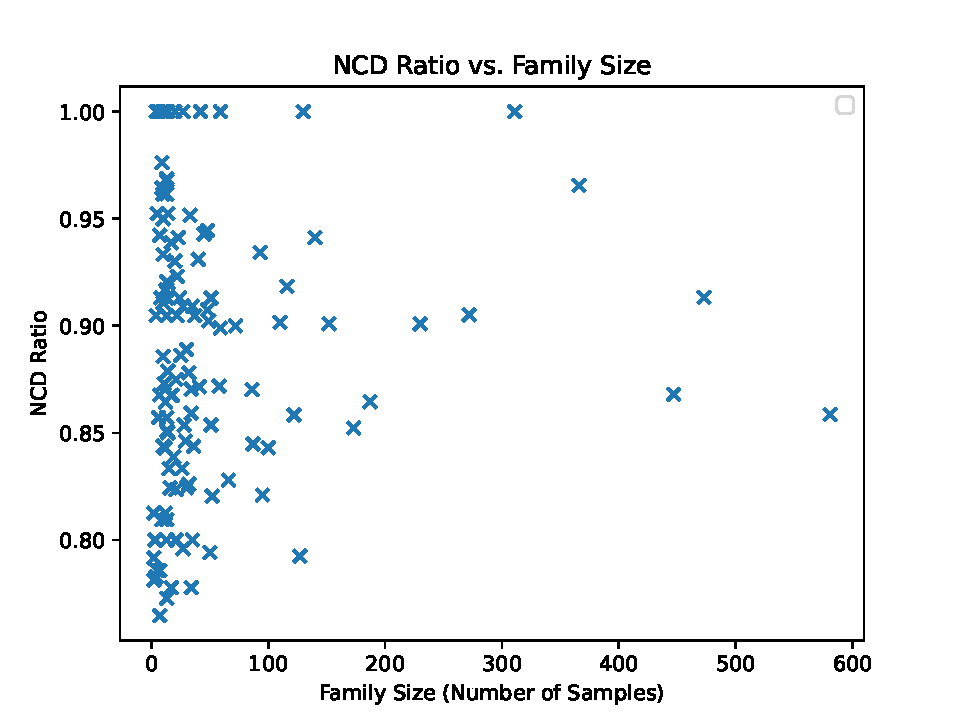
\includegraphics[width=.9\linewidth]{fig2/ncd-ratio-vs-family-size.pdf}
\caption{NCD Ratio denotes the fraction of average numbers of case distinctions in prime implicants divided by the average number of case distinctions by leaf nodes. The NCD ratios of all classes are scattered over the number of samples in each class (Family Size)}
\label{fig:ncdr-vs-size}
\end{figure}

\begin{figure}
\begin{minipage}{.49\linewidth}
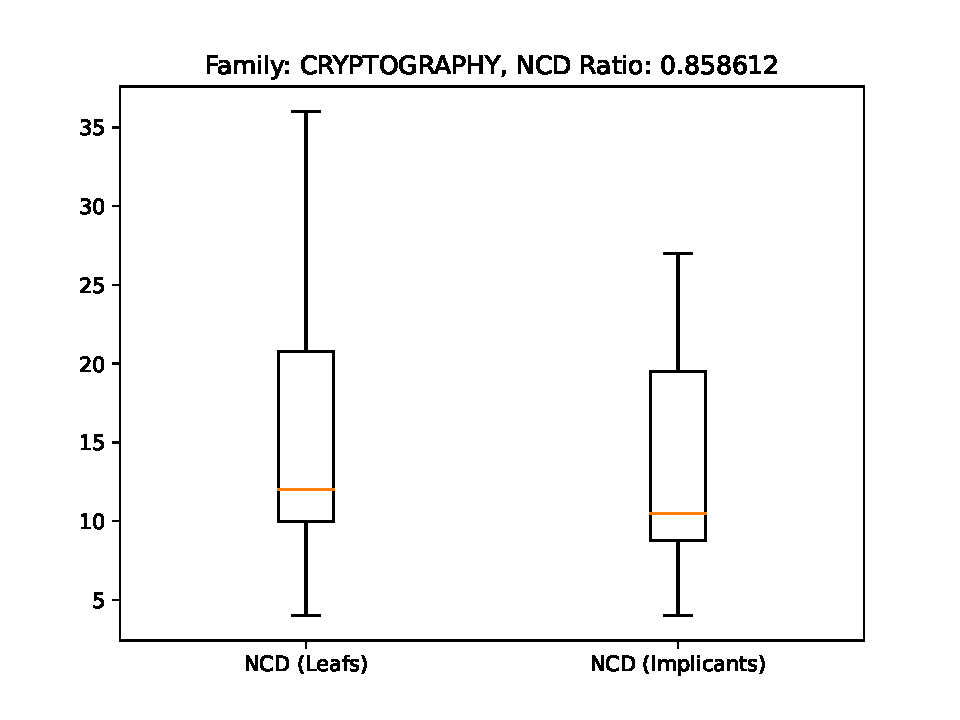
\includegraphics[width=\linewidth]{fig2/dc-crypto.pdf}\\
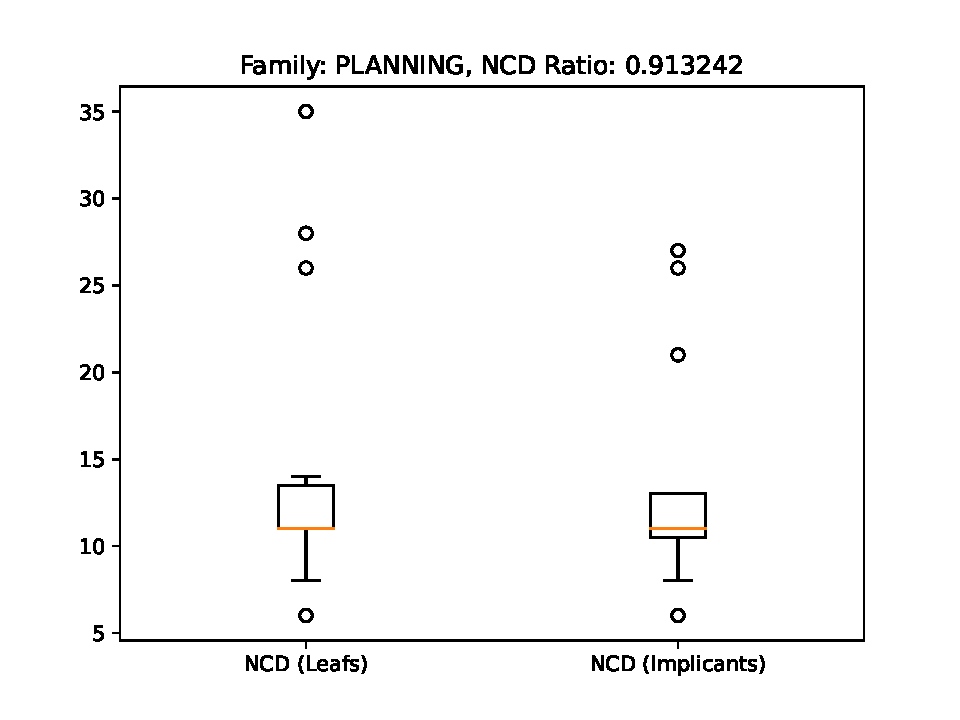
\includegraphics[width=\linewidth]{fig2/dc-planning.pdf}
\end{minipage}
\begin{minipage}{.49\linewidth}
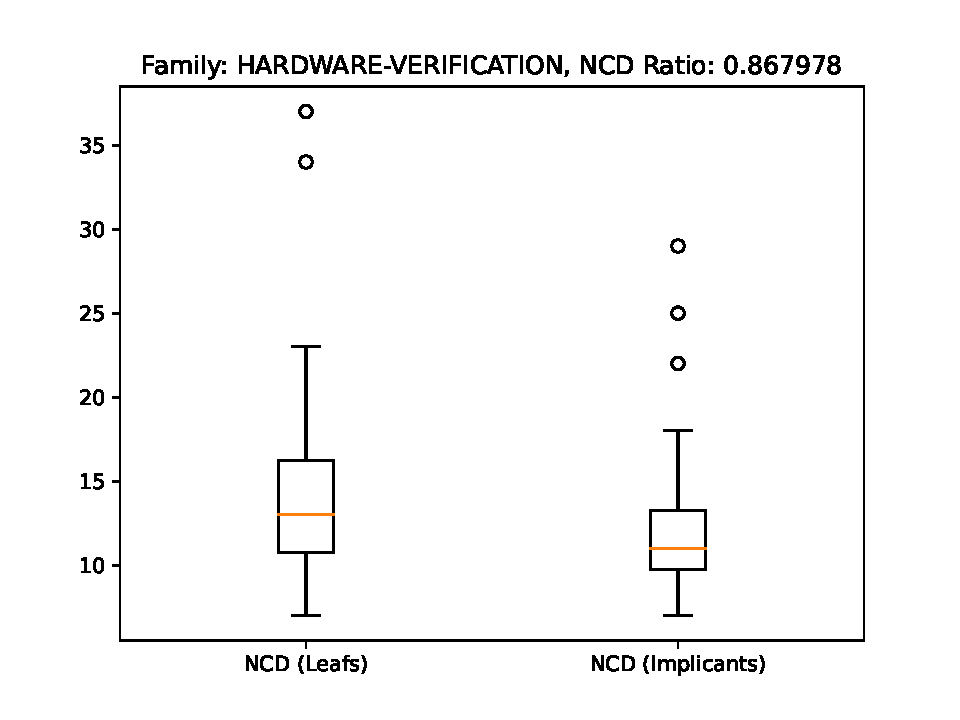
\includegraphics[width=\linewidth]{fig2/dc-hardwareverification.pdf}\\
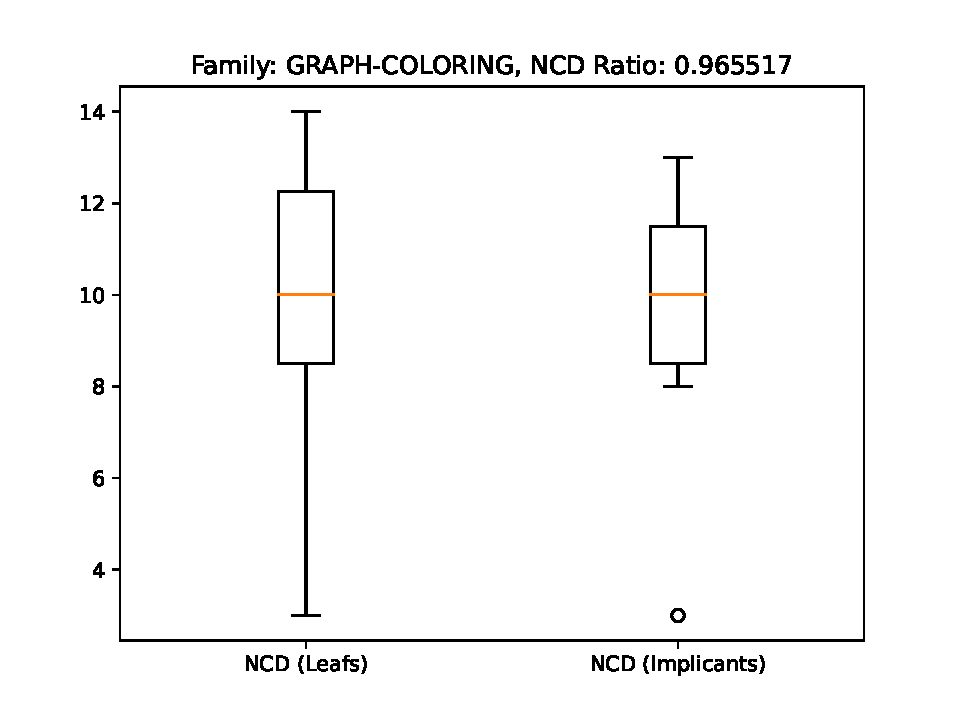
\includegraphics[width=\linewidth]{fig2/dc-graphcoloring.pdf}
\end{minipage}
\caption{NCD denotes the absolute number of case distinctions in prime implicants (Implicants) and leaf nodes (Leafs). 
The classifier was trained to separate instances by their family. 
The plots depict the distributions of these values for the four largest classes \emph{cryptography},  \emph{hardeware-verification}, \emph{planning} and \emph{graph-coloring}.}
\label{fig:eval:families}
\end{figure}

We trained a decision tree classifier to predict instance families for instances of SAT Competitions~2002 - 2021. 
Benchmarks of SAT Competitions~2004 and~2005 were missing. 
We excluded instances of random instance families and the agile tracks. 
That left us with a total 6647 instances of 124 distinct instance families. 
We train a decision tree classifier to predict the family of an instance given the instance features described in Sections~\ref{sec:data:base} and~\ref{sec:data:gate}. 
The accuracy of the classifier in a cross-validation experiment leaving out 20\% of the instances as a testing set is around $94\%$. 

Figure~\ref{fig:eval:families} depicts the explanation sizes for four exemplary families in terms of the leaf nodes (blue) and the prime implicants (orange). 
The x-axis shows the number of case distinctions, which corresponds to the node depths in terms of the leaf nodes and the number of decoded case distinctions in case of the prime implicants. 
The y-axis shows the number of training samples selected by the respective case distinctions. 
Using prime implicants we need less case distinctions to explain a classification result, while at the same time covering more samples than with leaf nodes. 


\subsubsection{Small Portfolios Classifier} 

\begin{figure}
\begin{minipage}{.49\linewidth}
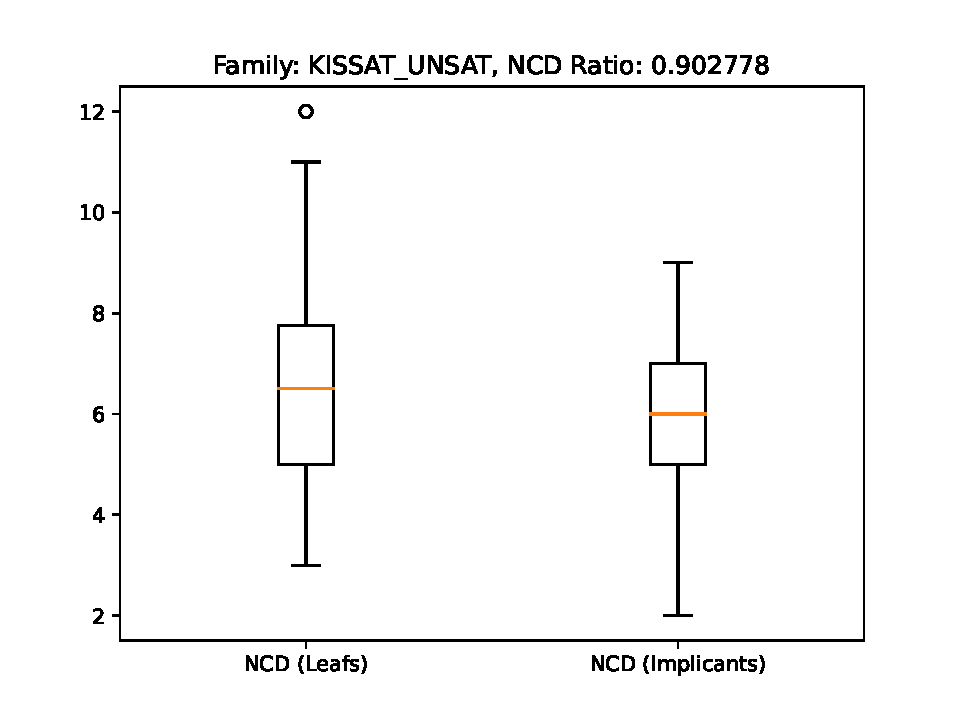
\includegraphics[width=\linewidth]{fig2/dc2-kissat-unsat.pdf}
\end{minipage}
\begin{minipage}{.49\linewidth}
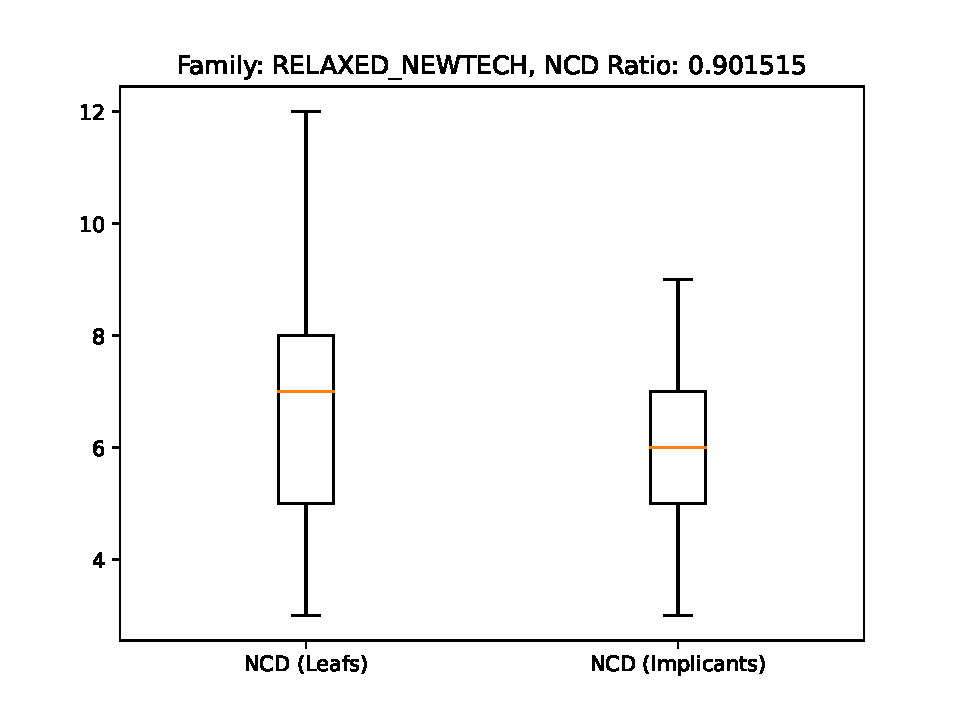
\includegraphics[width=\linewidth]{fig2/dc2-relaxed-newtech.pdf}
\end{minipage}
\caption{Number of Case Distinctions (NCD) and Number of Covered Training Samples (Cov.) for \emph{Prime Implicants} (Implicants) vs. \emph{Leaf Nodes} (Leafs). The classifier was trained to separate instances for \emph{Kissat Unsat} from instances for \emph{Relaxed NewTech} (by solver speed).}
\label{fig:eval:portfolio}
\end{figure}

Froleyks et al. report on best small portfolios drawn from solvers of SAT Competition~2020~\cite{Froleyks:2021:SC2020}. 
The best performing 2-portfolio in terms of its VBS score for the 400 instances in the SAT Competition~2020 benchmarks is \textsf{Kissat unsat} and \textsf{Relaxed newTech}. 

We train a decision tree classifier to predict the fastest solver for an instance given the instance features described in Sections~\ref{sec:data:base} and~\ref{sec:data:gate}. 
The accuracy of the classifier in a cross-validation experiment leaving out 20\% of the instances as a testing set is around $68\%$. 
Figure~\ref{fig:eval:portfolio} shows that also in this case, with prime implicants we need less case distinctions while at the same time covering more samples when using prime implicants as opposed to leaf nodes.

\begin{figure}
\begin{minipage}{.49\linewidth}
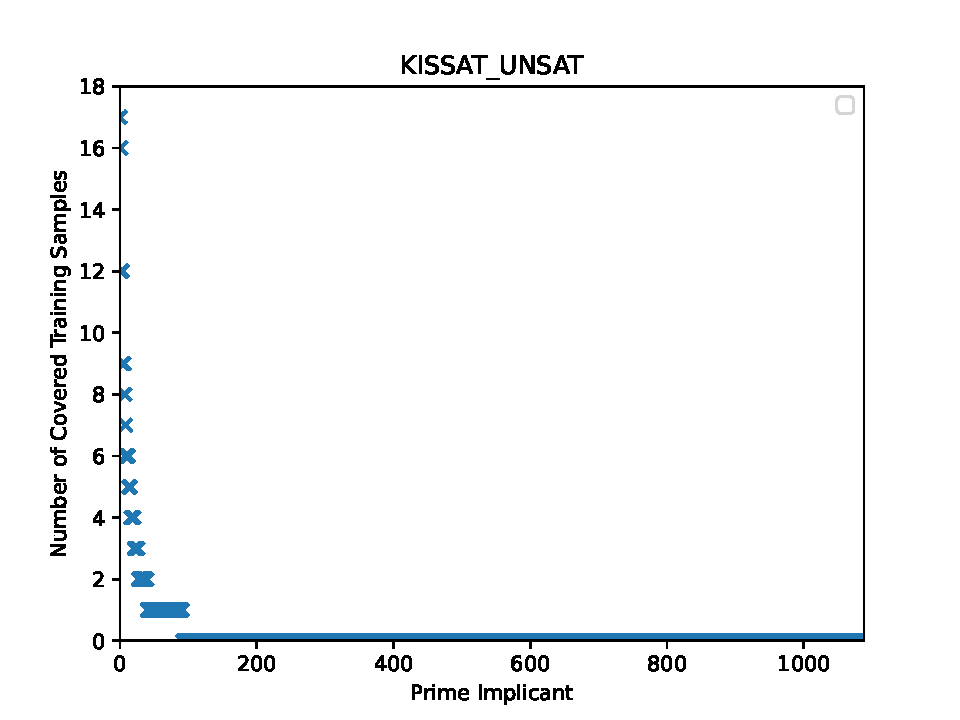
\includegraphics[width=\linewidth]{fig2/random-forest-2-kissat-unsat.pdf}
\end{minipage}
\begin{minipage}{.49\linewidth}
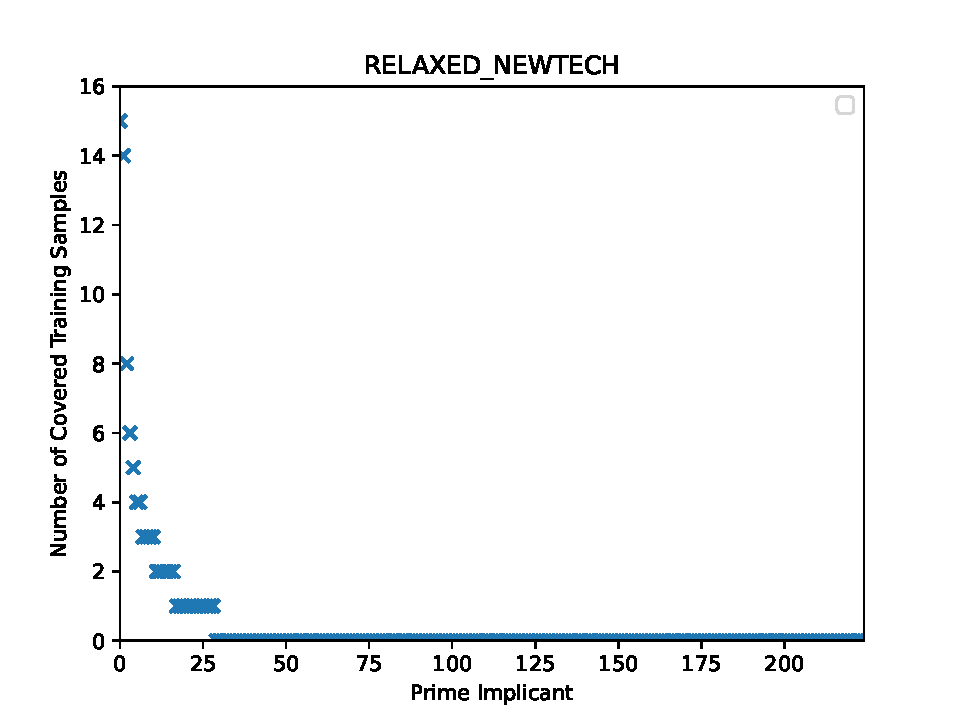
\includegraphics[width=\linewidth]{fig2/random-forest-2-relaxed-newtech.pdf}
\end{minipage}
\caption{Number of Covered Training Samples for all \emph{Prime Implicants}. The classifier was trained to separate instances for \emph{Kissat Unsat} from instances for \emph{Relaxed NewTech} (by solver speed).}
\label{fig:eval:portfolio-rf}
\end{figure}

We also train a random forest classifier consisting of only 2 decision trees for the same data. 
For this classifer, the accuracy in a cross-validation experiment leaving out 20\% of the instances as a testing set raises to around $76\%$. 
Figure~\ref{fig:eval:portfolio-rf} shows the number of training samples for each prime implicant of the two classes. 
We observe a large number of prime implicants with zero training samples. 
This is due to ``spurious'' valid tuples of leaf nodes emerging in the random forest. 
The total number of leaf node combinations in this forest is $1518$. 
The number of valid tuples determined by our encoding algorithm is $1312$ (cf. Section~\ref{sec:valid-tuples}). 
The \textsf{Kissat unsat} class encompasses a total of $1088$ prime implicants. 
The \textsf{Relaxed newTech} class encompasses a total of $224$ prime implicants. 
$92$ of those prime implicants encompass training samples of which only $40$ cover more than $1$ training sample. 

We also train a random forest classifier consisting of only 3 decision trees for the same data. 
For this classifer, the accuracy in a cross-validation experiment leaving out 20\% of the instances as a testing set raises to around $78\%$. 
In this scenario, we have a total of $66792$ leaf node combinations, of which $48880$ are valid combinations, i.e., they are reachable by some combination of values in the feature space (cf. Section~\ref{sec:valid-tuples}). 
The \textsf{Kissat unsat} class encompasses a total of $27807$ prime implicants of which only $104$ prime implicants encompass training samples and only $37$ of the prime implicants encompass more than one training sample. 
The \textsf{Relaxed newTech} class encompasses a total of $21073$ prime implicants of which only $81$ prime implicants encompass training samples and only $31$ of the prime implicants encompass more than one training sample. 

%%%%%%%
\section{Conclusion}
\label{sec:conclusion}

Our evaluation shows that with prime implicants, we indeed need less case distinctions while at the same time covering more samples for explaining classification results. 
Calculating prime implicants has the advantage that we can extract useful information such as the smallest prime implicant covering most of the samples. 
This can for example be used to only calculate a small subset of the features for \emph{selecting solver configurations}. 
Moreover, specific prime implicants can become subject to further research questions, e.g., to reason about the \emph{imposed taxonomy} or for evaluating \emph{biases in benchmarks}. 

One problem for our approach is the growing number of interval thresholds in random forests. 
In initial experiments with the random forest encoding, we see a large number of prime implicants which is not represented by a sample in the training set, i.e, we discover a large number of valid leaf tuples in the random forest which is actually empty (in terms of training samples) but would still produce a classification result for yet unseen samples matching the imposed case distinctions. 
Our initial implementation of the random forest encoding described in this paper seemed only feasible for random forest of up to 3 desicion trees. 
One reason for this can also be seen in the large number of ``spurious'' valid leaf \emph{tuples}. 

We assume that the number of valid leaf tuples could be reduced by reducing the allowed feature thresholds, e.g., through rounding, in the implementation of the classifier. 
This would reduce the number of intervals for each feature and could thus positively impact the number of valid nodes due to less implicants with zero training samples. 
This could in turn also positively impact the performance of our approach and lead to more expressive implicants for random forests. 
We also intend to implement and analyze the encoding for random forests which we described in the footnote of Section~\ref{sec:approach:rf}. 

In future work, we want to analyze benchmark taxonomies in greater detail under inclusion of new features, e.g., graph modularity or clustering based features~\cite{Ansotegui:2019:Community,Li:2021:Hierarchical}. 
We will also study feature importance measures and generalization power based on prime implicants. 
Moreover, we will evaluate portfolio performance with solver selection based on only a few prime implicants. 

%%%%%%%
\bibliography{main}

\end{document}




